\chapter{Etiqueta monástica}
\label{etiquette}

\section{La Reverencia y posturas}

Inclinarse, o postrarse ante aquellas cosas que uno considera dignas del mayor respeto, ya sean los mayores o maestros, objetos sagrados o lugares sagrados, es una parte milenaria de la cultura budista y una de las muchas y hermosas formas de etiqueta budista.

Realizada de forma correcta y consciente, la reverencia no es solo un ritual vacío que implica rebajarse ante imágenes religiosas por una aceptación ciega de la costumbre. Más bien, es una forma de mostrar fe, respeto y gratitud hacia aquello que es verdaderamente digno de tal veneración. Además, es un acto de humildad, una cualidad que es a la vez una bendición para los demás y que inclina la propia mente hacia los ideales y aspiraciones espirituales que esos objetos representan. Inclinarse ante la Triple Joya es elevar el propio corazón y la propia mente.

La forma y el método correctos para hacer la reverencia son los siguientes:

\subsection{La reverencia o postración de los cinco puntos}

El término 'postración de cinco puntos' se refiere a los cinco puntos del cuerpo que hacen contacto con el suelo cuando se realiza una reverencia. Son la frente, ambos codos y ambas rodillas.

\captionsetup{font=small, labelformat=empty, position=above}

\subsection{La postura preparatoria de la Reverencia:}

\begin{figure}[h]
	\centering
	
	\begin{minipage}{0.49\textwidth}
		\centering
		\caption{Los hombres se arrodillan en cuclillas con las palmas de ambas manos apoyadas en los muslos, como se muestra a continuación.}
		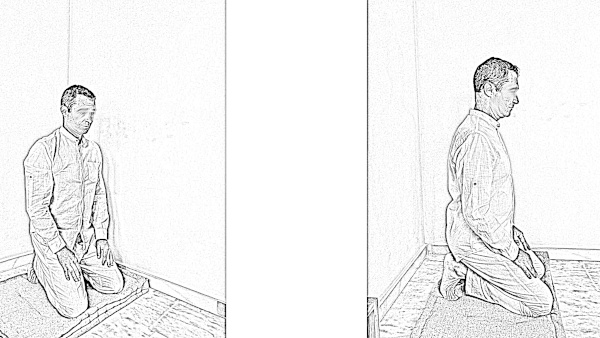
\includegraphics[scale=0.25,width=1\textwidth]{prep-man-ai.jpg}
		
	\end{minipage}
	\hfill
	\begin{minipage}{0.49\textwidth}
		\centering
		\caption{Las mujeres adoptan la misma postura, pero con los pies metidos debajo de ellas, como se muestra a continuación.}
		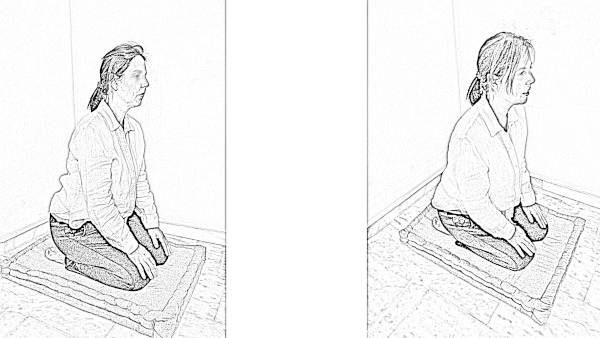
\includegraphics[scale=0.25,width=1\textwidth]{prep-woman-ai.jpg}
		
	\end{minipage}
	
\end{figure}


\subsection{El 'Añjali'}

Junta las palmas de las manos a la altura del pecho, apuntando hacia arriba en un ángulo de cuarenta y cinco grados con los dedos cerrados.
\begin{figure}[h]
	\centering
	
	\begin{minipage}{0.49\textwidth}
		\centering
		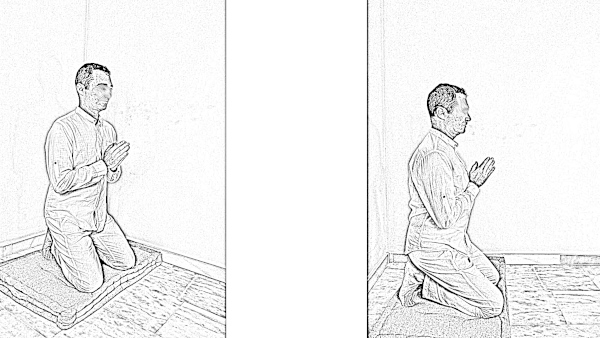
\includegraphics[scale=0.25,width=1\textwidth]{anjali-man-ai.jpg}
		%\label{fig:1}
	\end{minipage}
	\hfill
	\begin{minipage}{0.49\textwidth}
		\centering
		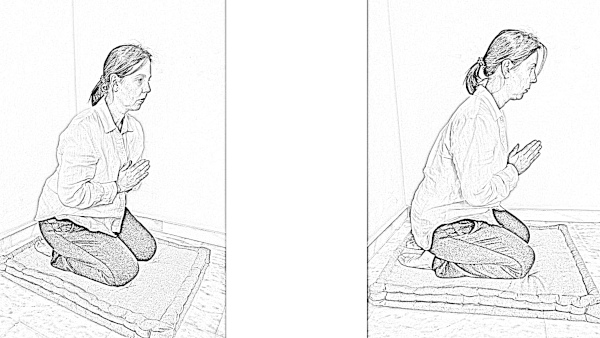
\includegraphics[scale=0.25,width=1\textwidth]{anjali-woman-ai.jpg}
		%\label{fig:2}
	\end{minipage}
	
\end{figure}

\subsection{El 'Vandana'}

Lleva el añjali (palmas cerradas) hasta la frente de modo que los pulgares se coloquen entre las cejas y las puntas de los dedos índice estén en la línea del cabello.

\begin{figure}[h]
	\centering
	
	\begin{minipage}{0.49\textwidth}
		\centering
		\caption{Los hombres mantienen la cabeza recta.}
		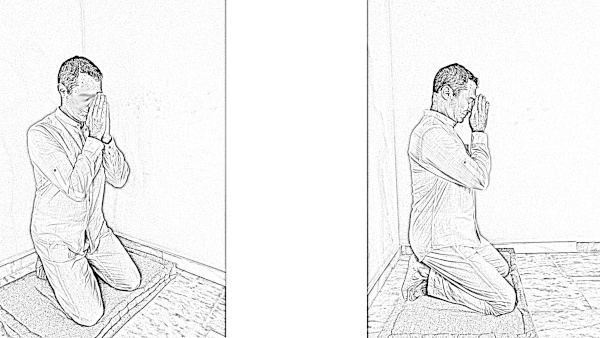
\includegraphics[scale=0.25,width=1\textwidth]{vandana-man-ai.jpg}
		%\label{fig:1}
	\end{minipage}
	\hfill
	\begin{minipage}{0.49\textwidth}
		\centering
		\caption{Las mujeres inclinan la cabeza ligeramente hacia adelante.}
		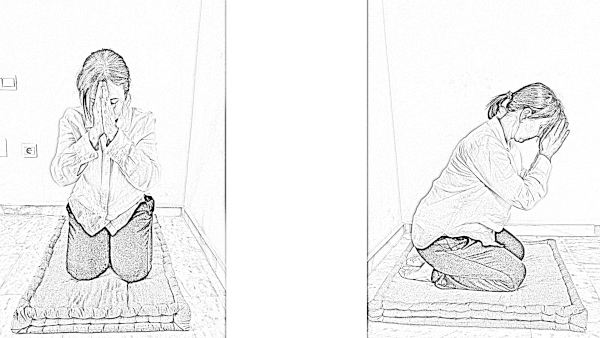
\includegraphics[scale=0.25,width=1\textwidth]{vandana-woman-ai.jpg}

		%\label{fig:2}
	\end{minipage}
\end{figure}
\enlargethispage{3\baselineskip}
\subsection{El 'Abhivada'}
Manteniendo la espalda recta, inclínate llevando la frente al suelo de modo que toque el espacio entre las palmas (aproximadamente a una distancia de un palmo), que ahora estarán boca abajo, planas sobre el suelo.
\begin{figure}[h]
	\centering
	\begin{minipage}{0.40\textwidth}
		\centering
		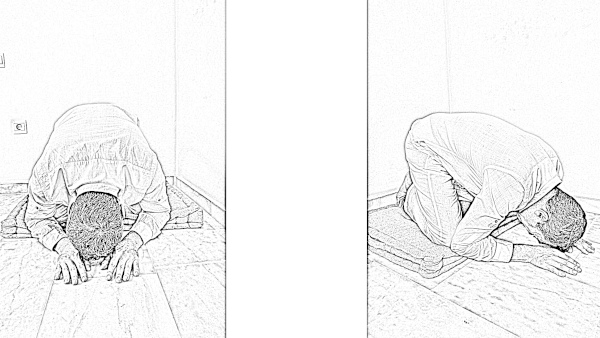
\includegraphics[scale=0.2,width=1\textwidth]{abhivada-man-ai.jpg}
		\caption{Los hombres mantienen los codos y las rodillas alineados y tocándose.}
		%\label{fig:1}
	\end{minipage}
	\hfill
	\begin{minipage}{0.40\textwidth}
		\centering
		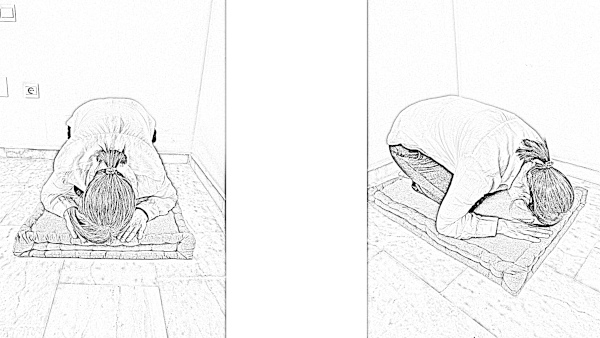
\includegraphics[scale=0.2,width=1\textwidth]{abhivada-woman-ai.jpg}
		\caption{Las mujeres colocan los codos a cada lado de las rodillas}
		%\label{fig:2}
	\end{minipage}
\end{figure}

\subsection{\thaiFont พับเพียบ 'papiyap'}

\thaiFont{'พับเพียบ'} \normalfont(pronunciado 'papiyap')es un término tailandés que se refiere a la postura tradicional que se adopta al cantar. Sentarse \thaiFont{'พับเพียบ'} \normalfont significa sentarse con las piernas dobladas a un lado, como se muestra en el diagrama a continuación. La postura de piernas cruzadas o 'loto' se reserva para la práctica formal de meditación. Sentarse con las piernas o los pies apuntando hacia una imagen de Buddha o un monje se considera irrespetuoso, ya que los pies son la parte más baja del cuerpo. Por lo tanto, \thaiFont{'พับเพียบ'} \normalfont es una postura apropiada para asumir mientras se canta. Sin embargo, cuando se cantan los versos de homenaje a la Triple Joya (Sección 1-Vol. 1), uno se arrodilla sobre sus talones. 
\enlargethispage{3\baselineskip}
\begin{figure}[h]
	\centering
	
	\begin{minipage}{0.49\textwidth}
		\centering
		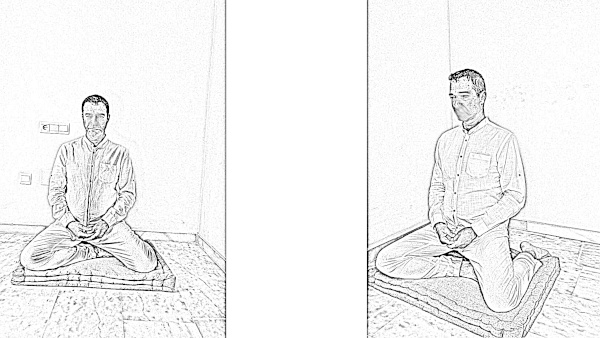
\includegraphics[scale=0.25,width=1\textwidth]{papiap-man-ai.jpg}
		\caption{Los hombres se sientan con una pierna doblada a un lado y la otra pierna cruzada frente a ellos, con la planta del pie tocando la rodilla.}
		%\label{fig:1}
	\end{minipage}
	\hfill
	\begin{minipage}{0.49\textwidth}
		\centering
		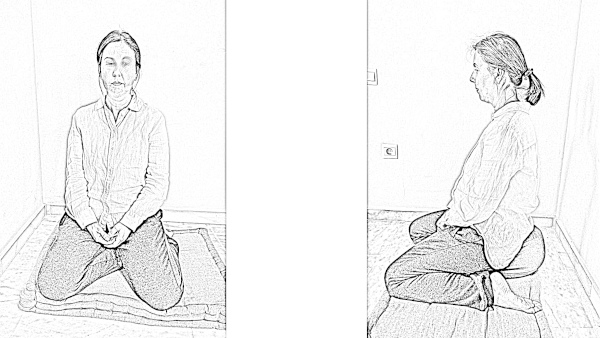
\includegraphics[scale=0.25,width=1\textwidth]{papiap-woman-ai.jpg}
		\caption{Las mujeres se sientan con una pierna doblada a un lado, pero con la otra pierna doblada debajo de ellas, manteniendo las rodillas juntas. Tradicionalmente, las mujeres no se sientan con las rodillas muy separadas mientras cantan como lo hacen los hombres.}
		%\label{fig:2}
	\end{minipage}
	
\end{figure}

\subsection{Cambio de postura}


No está mal cambiar de postura cuando el dolor se agudiza, pero debe hacerse de manera educada. La mejor manera de cambiar de postura, ya sea sentado en meditación o mientras se canta, es cambiar la posición de las piernas desde atrás en lugar de desde adelante, inclinándose hacia adelante y usando una mano en el suelo para apoyarse.
\clearpage

\section{Etiqueta general en el monasterio y la sala de meditación}

El monasterio y, en particular, la sala principal de meditación son un espacio sagrado. La sala de meditación (sala Uposatha) siempre debe proporcionar tanto a la comunidad monástica como a la laica un entorno adecuado y propicio para la práctica de virtud, meditación y desarrollo de sabiduría. Hay ciertos tipos de comportamiento que contribuyen a una atmósfera de buena práctica espiritual y reflexión tranquila, y otros tipos de comportamiento que pueden destruirla rápidamente. Por lo tanto, es importante que cualquier persona que entre en el monasterio y, por extensión, en la sala de meditación, sea considerada respecto a cómo su comportamiento puede estar afectando a quienes le rodean. Esto beneficiará tanto a la propia práctica de Sati, como al entorno del monasterio en su conjunto.

Cuando entre en la sala principal, observe las siguientes prácticas:


\begin{enumerate}
\item Si es necesario hablar con alguien, es mejor salir a hacerlo. O al menos hágalo lo más silenciosa y brevemente posible, para no molestar a las personas a su alrededor que podrían estar tratando de meditar.

\item No se permiten sombreros, capuchas, gorros, zapatos, comida ni bebidas (incluidas botellas de agua) en la sala.

\item Se agradecería que los padres con bebés o niños pequeños sacaran a sus hijos de la sala si empiezan a llorar o a comportarse de forma incontrolable durante las sesiones de meditación y discursos de Dhamma.

\item Solo se pueden tomar fotos y vídeos con el permiso directo del monje de mayor antigüedad.

\item El monasterio es un lugar de celibato. La separación de sexos se practica estrictamente durante los retiros de meditación, y se debe evitar cualquier forma de contacto físico inadecuado con el sexo opuesto en cualquier lugar de los terrenos del monasterio.

\item Al entrar al monasterio, es importante vestir apropiadamente. Los hombres no deben caminar sin camisa y las mujeres deben evitar cualquier tipo de ropa que sea reveladora o inmodesta.

\item Por favor, no se siente apuntando con los pies hacia el altar ni hacia los monjes, ya que esto se considera una falta de respeto.

\item Por favor, no suba a la plataforma elevada frente al altar principal. Es un espacio reservado solo para la Saṅgha monástica.

\item Todos los teléfonos móviles o cualquier otro dispositivo eléctrico que pueda hacer ruido deben dejarse fuera de la sala o apagarse antes de entrar en ella.

\item Estas normas se aplican no solo a la sala principal de meditación, sino a cualquier edificio del monasterio donde se celebren discursos de Dhamma o se practique la meditación.
\end{enumerate}
Una actitud básica de moderación y respeto es todo lo que se necesita.

Gracias




